\documentclass[12pt]{beamer}
\usetheme{Boadilla}
\usepackage{booktabs}
\usepackage{multirow}
\usepackage{enumitem}
\usepackage{tikz}

\newcommand{\E}{\mathbb{E}}
\usefonttheme{professionalfonts}
\usepackage{pgfplots}
\pgfplotsset{compat=1.18}
\renewcommand{\arraystretch}{1.25}
\usetikzlibrary{trees}
\title[ECON2843]{Lecture 20}
\subtitle{Part 4 Analysis of Variance}
\date{}
\usepackage{amsmath,amssymb,mathtools,wasysym}
\begin{document}
	\begin{frame}
		\titlepage

	\end{frame}
	\begin{frame}
		\vspace{1cm}
		\centering
		{\color{blue}\large Chi-squared Test}
	\end{frame}

		
		\begin{frame}
			\frametitle{Tests for Categorical Data}
			
			\begin{itemize}[label={\color{blue}$\blacktriangleright$}]
				\item Testing population proportions can be thought of as making inferences about populations of categorical data with two categories.
				\begin{itemize}[label={\color{blue}$\blacktriangleright$}]
					\item For example, ``Coke'' and ``Pepsi''. We can denote Coke as a \emph{success}, Pepsi as a \emph{failure} and perform tests on the population proportion of successes, $p$.
				\end{itemize}
				\item Chi-squared tests are designed to make inferences about populations of categorical data with \emph{two or more} categories.
				\begin{itemize}[label={\color{blue}$\blacktriangleright$}]
					\item For example, ``Coke'', ``Pepsi'' and ``Dr Pepper''.
				\end{itemize}
			\end{itemize}
			
		\end{frame}
		\begin{frame}
			\frametitle{Chi-Squared Tests}
			
			\begin{enumerate}[label={\color{blue}\arabic{enumi}.}]
				\item Chi-squared goodness-of-fit test.
				\begin{itemize}[label={\color{blue}$\blacktriangleright$}]
					\item Used to analyze a population of categorical data arising from \emph{one} categorical variable with $k$ categories.
					\item Specifically, used to describe the population proportion of observations in each category.
				\end{itemize}
				
				\item Chi-squared test of a contingency table.
				\begin{itemize}[label={\color{blue}$\blacktriangleright$}]
					\item Used to analyze a population of categorical data arising from \emph{two} categorical variables with $r$ and $c$ categories, respectively.
					\item Specifically, used to determine whether the two categorical variables are \emph{independent}.
				\end{itemize}
			\end{enumerate}
			
		\end{frame}
		\begin{frame}
			\frametitle{College Example}
			
			\begin{itemize}[label={\color{blue}$\blacktriangleright$}]
				\item Suppose we surveyed a sample of 206 students and recorded the college in which they studied.
				\item The data is summarized below:
				
				\medskip
				
				\begin{center}
					\begin{tabular}{cccccc}
					\toprule
					College & Business & Arts & CS & Science & Law \\
					\midrule
					Count & 65 & 20 & 35 & 62 & 24 \\
					\bottomrule
				\end{tabular}
			\end{center}
				
				\medskip
				\item We want to test whether the population proportions of students in each college are equal.
			\end{itemize}
			
		\end{frame}
		\begin{frame}
			\frametitle{Hypotheses}
			
			\begin{itemize}[label={\color{blue}$\blacktriangleright$}]
				\item Let $p_1$, $p_2$, $p_3$, $p_4$ and $p_5$ denote the population proportion of students in Business, Arts, Computer Science, Science, and Law, respectively.
			\end{itemize}
			
			\medskip
			
			$H_0$ : Population proportions in each college are equal.
			\[\text{That is,} \quad p_1 = p_2 = p_3 = p_4 = p_5 = \frac{1}{5}\]
			
			$H_1$ : Not all population proportions are equal.
			
		\end{frame}
		\begin{frame}
			\frametitle{Test Statistic}
			
			\begin{itemize}[label={\color{blue}$\blacktriangleright$}]
				\item If we assume $H_0$ is true, what would be the expected count in each college?
				\item We would expect one-fifth of total students in each college, i.e., $\frac{1}{5} \times 206 = 41.2$ students.
			\end{itemize}
			
			\medskip
			
			\begin{center}
				\begin{tabular}{cccccc}
				\toprule
				College & Business & Arts & CS & Science & Law \\
				\midrule
				Observed & 65 & 20 & 35 & 62 & 24 \\
				Expected & 41.2 & 41.2 & 41.2 & 41.2 & 41.2 \\
				\bottomrule
			\end{tabular}
			\end{center}
			
		\end{frame}
		\begin{frame}
			\frametitle{Test Statistic}
			
			\begin{itemize}[label={\color{blue}$\blacktriangleright$}]
				\item If the observed counts are close to the expected counts, then that is evidence supporting $H_0$.
				
				\item If the observed counts are far from the expected counts, then that is evidence against $H_0$.
				
				\item So we need a test statistic that measures how close the observed counts are to the expected counts.
			\end{itemize}
			
		\end{frame}
		\begin{frame}
			\frametitle{Test Statistic}
			
			\begin{itemize}[label={\color{blue}$\blacktriangleright$}]
				\item The test statistic that we use is called the chi-squared goodness-of-fit statistic:
			\end{itemize}
			
			\medskip
			
			\[
			\chi^2 = \sum_{i=1}^k \frac{(f_i - e_i)^2}{e_i}
			\]
			
			\medskip
			
			where $k$ is the number of categories, $f_i$ are the observed counts and $e_i$ are the expected counts.
			
		\end{frame}
		\begin{frame}
			\frametitle{Test Statistic}
			
			\begin{itemize}[label={\color{blue}$\blacktriangleright$}]
				\item For our data:
			\end{itemize}
			
			\medskip
			
			\[
			\chi^2 = \sum_{i=1}^5 \frac{(f_i - e_i)^2}{e_i}
			\]
			\[
			= \frac{(65 - 41.2)^2}{41.2} + \frac{(20 - 41.2)^2}{41.2} + \frac{(35 - 41.2)^2}{41.2}
			\]
			\[
			\quad + \frac{(62 - 41.2)^2}{41.2} + \frac{(24 - 41.2)^2}{41.2}
			\]
			\[
			= 43.2718
			\]
			
		\end{frame}
		\begin{frame}
			\frametitle{Decision Rule}
			
			\begin{itemize}[label={\color{blue}$\blacktriangleright$}]
				\item A small $\chi^2$-statistic supports $H_0$, whereas a large $\chi^2$-statistic supports $H_1$.
				
				\item So we should reject $H_0$ when the $\chi^2$-statistic is large, meaning that this is an \emph{upper-tailed test}.
				
				\item The sampling distribution of this $\chi^2$-statistic is the \emph{chi-squared distribution} with $k-1$ degrees of freedom.
			\end{itemize}
			
		\end{frame}
		\begin{frame}
			\frametitle{Chi-Squared Distribution}
			
			\begin{itemize}[label={\color{blue}$\blacktriangleright$}]
				\item Another special continuous distribution.
				
				\item It has one parameter called the degrees of freedom.
				
				\item There is a $\chi^2$-table listing probabilities.
			\end{itemize}
			\vspace{0.5cm}
			\centering
			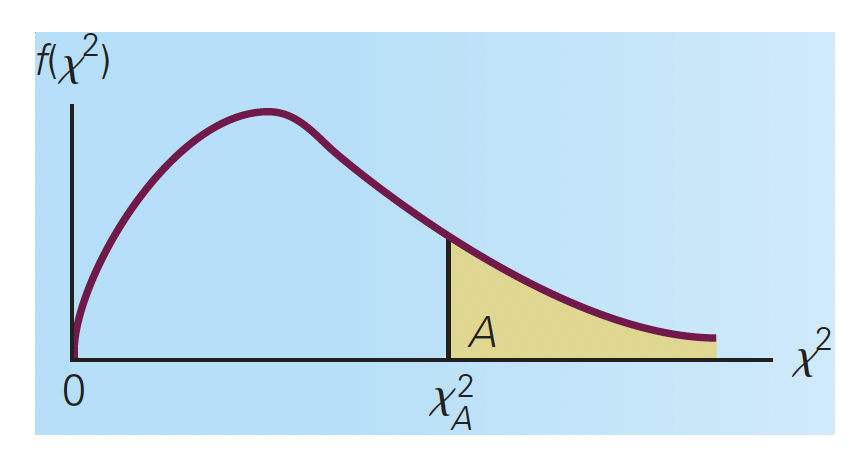
\includegraphics[width=8cm]{chidist.png}
		\end{frame}
		\begin{frame}
			\frametitle{Decision Rule and Conclusion}
			
			\begin{itemize}[label={\color{blue}$\blacktriangleright$}]
				\item Decision Rule:
				\begin{itemize}[label={\color{blue}$\blacktriangleright$}]
					\item We compare the $\chi^2$-statistic to a chi-squared distribution with $k-1=4$ degrees of freedom.
					\item For $\alpha = 5\%$, the critical value is 9.49, so the rejection region is $\chi^2 > 9.49$.
				\end{itemize}
				
				\item Conclusion:
				\begin{itemize}[label={\color{blue}$\blacktriangleright$}]
					\item Since $43.27 > 9.49$, our test statistic lies in the rejection region, so we reject $H_0$.
					\item Conclude that the population proportions of students in each college are not equal.
				\end{itemize}
			\end{itemize}
			
		\end{frame}
				\begin{frame}
			\frametitle{Decision Rule and Conclusion}
			\centering
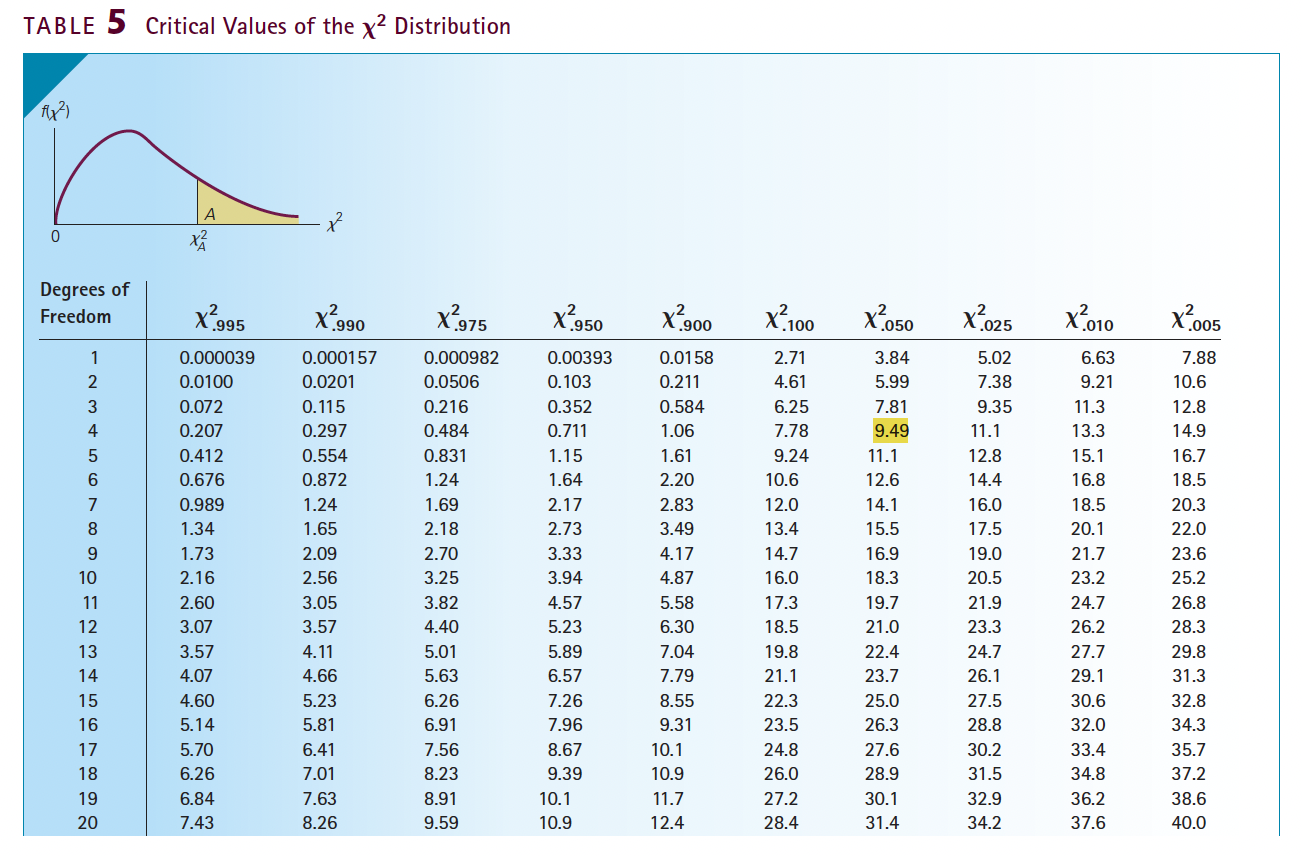
\includegraphics[width=11cm]{chitable.png}
			
		\end{frame}
		\begin{frame}
			\frametitle{Summary}
			
			\begin{itemize}[label={\color{blue}$\blacktriangleright$}]
				\item The \textbf{Chi-squared goodness-of-fit test} is used in the situation where we have \emph{one} categorical variable with $k$ categories.
				
				\item Hypotheses:
				
				\medskip
				$H_0$ : Population proportions in each category are given by some specified values.
				
				\medskip
				$H_1$ : At least one population proportion is not equal to its specified value.
			\end{itemize}
			
		\end{frame}
		\begin{frame}
			\frametitle{Summary}
			
			\begin{itemize}[label={\color{blue}$\blacktriangleright$}]
				\item Test statistic:
			\end{itemize}
			
			\medskip
			
			\[
			\chi^2 = \sum_{i=1}^k \frac{(f_i - e_i)^2}{e_i}
			\]
			
			\medskip
			
			where $k$ is the number of categories, $f_i$ are the observed counts in each category and $e_i$ are the expected counts (based on $H_0$) in each category.
			
		\end{frame}
		\begin{frame}
			\frametitle{Summary}
			
			\begin{itemize}[label={\color{blue}$\blacktriangleright$}]
				\item Decision rule and conclusion:
				\begin{itemize}[label={\color{blue}$\blacktriangleright$}]
					\item Compare $\chi^2$-statistic to a chi-squared distribution with $k-1$ degrees of freedom.
					\item At a significance level of $\alpha$, reject $H_0$ if $\chi^2 > \chi^2_{\alpha,k-1}$, where $\chi^2_{\alpha,k-1}$ is the critical value that cuts off $100\alpha\%$ in the upper tail of the chi-squared distribution with $k-1$ degrees of freedom.
				\end{itemize}
			\end{itemize}
			
		\end{frame}
		\begin{frame}
			\frametitle{Network Satisfaction Example}
			
			\begin{itemize}[label={\color{blue}$\blacktriangleright$}]
				\item A survey was performed within a company to assess the degree to which staff were satisfied with the computer network.
				
				\item Staff were classified as either administrative, technical or management.
				
				\item Responses were classified as either satisfied, neutral or dissatisfied.
			\end{itemize}
			
		\end{frame}
\begin{frame}
	\frametitle{Network Satisfaction Example}
	
	\medskip
		\centering
	\begin{tabular}{llcccc}

		\toprule
		& & \multicolumn{3}{c}{Group} &\multirow{2}{*}{Total}  \\
		& & Admin & Tech & Manage &\\
		\midrule
		\multirow{3}{*}{Response} & Satisfied & 37 & 11 & 35 & 83 \\
		& Neutral & 18 & 25 & 10 & 53 \\
		& Dissatisfied & 20 & 24 & 20 & 64 \\
		\midrule
		\multicolumn{2}{l}{Total} & 75 & 60 & 65 & 200 \\
		\bottomrule
	\end{tabular}
	
\end{frame}
\begin{frame}
	\frametitle{Network Satisfaction Example}
	
	\begin{itemize}[label={\color{blue}$\blacktriangleright$}]
		\item Test whether there are half as many staff who are satisfied than staff who are either neutral or dissatisfied.
		
		\item That is, for every staff member who is satisfied, there are two who are neutral or dissatisfied.
	\end{itemize}
	
	\medskip
	
	\begin{center}
		\begin{tabular}{lc}
			\toprule
			Response & Total \\
			\midrule
			Satisfied & 83 \\
			Neutral & 53 \\
			Dissatisfied & 64 \\
			\midrule
			Total & 200 \\
			\bottomrule
		\end{tabular}
	\end{center}
	
\end{frame}
\begin{frame}
	\frametitle{Hypotheses}
	
	$H_0$ : There are half as many staff satisfied with the network than not (either neutral or dissatisfied).
	
	\medskip
	\hspace*{1em} That is, \quad $p_\text{sat} = \frac{1}{3}$ \quad and \quad $p_\text{not-sat} = \frac{2}{3}$
	
	\medskip
	$H_1$ : The population proportions do not match that given above.
	
\end{frame}
\begin{frame}
	\frametitle{Hypotheses}
	
	\begin{itemize}[label={\color{blue}$\blacktriangleright$}]
		\item How did we get the probabilities for $H_0$?
		
		\item The question asked us to test whether the ratio of satisfied to not-satisfied staff was 1 to 2.
		
		\item To convert the ratio 1 : 2 to probabilities, add together the two numbers in the ratio and use that as the denominator.
		
		\item That is, $p_\text{sat} = \frac{1}{3}$ and $p_\text{not-sat} = \frac{2}{3}$.
	\end{itemize}
	
\end{frame}
\begin{frame}
	\frametitle{Test Statistic}
	
	\begin{itemize}[label={\color{blue}$\blacktriangleright$}]
		\item First calculate the expected counts:
	\end{itemize}
	
	\medskip
	
	\begin{center}
		\begin{tabular}{lcr}
			\toprule
			Response & Observed & Expected \\
			\midrule
			Satisfied & 83 & $200 \times \frac{1}{3} = 66.67$ \\
			Neutral or Dissatisfied & 117 & $200 \times \frac{2}{3} = 133.33$ \\
			\midrule
			Total & 200 & 200 \\
			\bottomrule
		\end{tabular}
	\end{center}
	
\end{frame}
\begin{frame}
	\frametitle{Test Statistic}
	
	\begin{itemize}[label={\color{blue}$\blacktriangleright$}]
		\item Then calculate the $\chi^2$-statistic:
	\end{itemize}
	
	\medskip
	
	\[
	\chi^2 = \sum_{i=1}^2 \frac{(f_i - e_i)^2}{e_i}
	\]
	\[
	= \frac{(83 - 66.67)^2}{66.67} + \frac{(117 - 133.33)^2}{133.33}
	\]
	\[
	= 6.0025
	\]
	
\end{frame}
\begin{frame}
	\frametitle{Decision Rule and Conclusion}
	
	\begin{itemize}[label={\color{blue}$\blacktriangleright$}]
		\item Decision rule:
		\begin{itemize}[label={\color{blue}$\blacktriangleright$}]
			\item Compare to a chi-squared distribution with $k-1=1$ degree of freedom.
			\item Reject $H_0$ at the 5\% significance level if $\chi^2 > \chi^2_{0.05,1} = 3.84$ (from table).
		\end{itemize}
		
		\item Conclusion:
		\begin{itemize}[label={\color{blue}$\blacktriangleright$}]
			\item Since $6.0025 > 3.84$, reject $H_0$ and conclude that there are not half as many satisfied staff as there are neutral or dissatisfied staff.
		\end{itemize}
	\end{itemize}
	
\end{frame}
\begin{frame}
	\frametitle{Chi-Squared Test of a Contingency Table}
	
	\begin{itemize}[label={\color{blue}$\blacktriangleright$}]
		\item Contingency table:
		\begin{itemize}[label={\color{blue}$\blacktriangleright$}]
			\item A cross-classification table of counts that summarizes the joint distribution of two categorical variables, each with a finite number of categories.
		\end{itemize}
		
		\item Chi-squared test of a contingency table:
		\begin{itemize}[label={\color{blue}$\blacktriangleright$}]
			\item Used to determine whether two categorical variables are independent. That is, to determine whether the distribution of one categorical variable is the same across all categories of the other categorical variable.
		\end{itemize}
	\end{itemize}
	
\end{frame}
\begin{frame}
	\frametitle{College Example}
	
	\begin{itemize}[label={\color{blue}$\blacktriangleright$}]
		\item Let's go back to the example where we surveyed 206 students and recorded the college in which they studied.
		
		\item Suppose now we also recorded whether each student was male or female.
		
		\item Now we have two categorical variables.
	\end{itemize}
	
\end{frame}
\begin{frame}
	\frametitle{College Example}
	
	\begin{center}
		\begin{tabular}{lccc}
			\toprule
			& Female & Male & Total \\
			\midrule
			Arts & 6 & 14 & 20 \\
			Business & 33 & 32 & 65 \\
			CS & 9 & 26 & 35 \\
			Law & 15 & 9 & 24 \\
			Science & 33 & 29 & 62 \\
			\midrule
			Total & 96 & 110 & 206 \\
			\bottomrule
		\end{tabular}
	\end{center}
	
\end{frame}
\begin{frame}
	\frametitle{Hypotheses}
	
	$H_0$ : College and gender are independent.
	\medskip
	
	\hspace*{2em}That is, the proportion of females is the same across all colleges.
	
	\bigskip
	
	$H_1$ : College and gender are not independent.
	\medskip
	
	\hspace*{2em}That is, the proportion of females differs across colleges.
	
\end{frame}
\begin{frame}
	\frametitle{Test Statistic}
	
	\begin{itemize}[label={\color{blue}$\blacktriangleright$}]
		\item Very similar to the chi-squared goodness-of-fit statistic:
	\end{itemize}
	
	\medskip
	
	\[
	\chi^2 = \sum_{i=1}^r \sum_{j=1}^c \frac{(f_{ij} - e_{ij})^2}{e_{ij}}
	\]
	
	\medskip
	
	where $r$ and $c$ are the number of rows and columns, respectively, in the table, and $f_{ij}$ and $e_{ij}$ are the observed and expected counts, respectively, for the cell in the $i$th row and $j$th column of the table.
	
\end{frame}
\begin{frame}
	\frametitle{Expected Counts}
	
	\begin{itemize}[label={\color{blue}$\blacktriangleright$}]
		\item But the expected counts are calculated differently.
		
		\item Remember that to calculate the test statistic we assume $H_0$ is true.
		
		\item Under $H_0$, the two categorical variables are independent.
		
		\item Expected counts are calculated from the margins of the table and are based on the independence of discrete random variables.
	\end{itemize}
	
\end{frame}
\begin{frame}
	\frametitle{Expected Counts}
	
	\begin{itemize}[label={\color{blue}$\blacktriangleright$}]
		\item If the variables are independent, then the joint probability of falling in the $(i, j)$th cell in the table is equal to:
		
		\medskip
		\[
		p(i,j) = p_r(i) \times p_c(j)
		\]
		
		\item But the marginal probabilities are equal to:
		
		\medskip
		\[
		p_r(i) = \frac{\text{$i$th row total}}{\text{sample size}}
		\]
		\[
		p_c(j) = \frac{\text{$j$th column total}}{\text{sample size}}
		\]
	\end{itemize}
	
\end{frame}
\begin{frame}
	\frametitle{Expected Counts}
	
	\begin{itemize}[label={\color{blue}$\blacktriangleright$}]
		\item Therefore, the expected counts are given by:
	\end{itemize}
	
	\medskip
	
	\begin{align*}
		e_{ij} &= \text{sample size} \times p(i,j) \\
		&= \text{sample size} \times p_r(i) \times p_c(j) \\
		&= \text{sample size} \times \frac{\text{$i$th row total}}{\text{sample size}} \times \frac{\text{$j$th column total}}{\text{sample size}} \\
		&= \frac{\text{$i$th row total} \times \text{$j$th column total}}{\text{sample size}}
	\end{align*}
	
\end{frame}
\begin{frame}
	\frametitle{Expected Counts}
	
	\begin{center}
		\begin{tabular}{lccc}
			\toprule
			& Female & Male & Total \\
			\midrule
			Arts & $\frac{20 \times 96}{206} = 9.32$ & $\frac{20 \times 110}{206} = 10.68$ & 20 \\[2ex]
			Business & $\frac{65 \times 96}{206} = 30.29$ & $\frac{65 \times 110}{206} = 34.71$ & 65 \\[2ex]
			CS & $\frac{35 \times 96}{206} = 16.31$ & $\frac{35 \times 110}{206} = 18.69$ & 35 \\[2ex]
			Law & $\frac{24 \times 96}{206} = 11.18$ & $\frac{24 \times 110}{206} = 12.82$ & 24 \\[2ex]
			Science & $\frac{62 \times 96}{206} = 28.89$ & $\frac{62 \times 110}{206} = 33.11$ & 62 \\[2ex]
			\midrule
			Total & 96 & 110 & 206 \\
			\bottomrule
		\end{tabular}
	\end{center}
	
\end{frame}
\begin{frame}
	\frametitle{Test Statistic}
	
	\begin{itemize}[label={\color{blue}$\blacktriangleright$}]
		\item For our data,
	\end{itemize}
	
	\medskip
	
	\[
	\chi^2 = \sum_{i=1}^r \sum_{j=1}^c \frac{(f_{ij} - e_{ij})^2}{e_{ij}}
	\]
	\[
	= \frac{(6 - 9.32)^2}{9.32} + \frac{(33 - 30.29)^2}{30.29} + \cdots
	\]
	\[
	\cdots + \frac{(29 - 33.11)^2}{33.11}
	\]
	\[
	= 12.3361
	\]
	
\end{frame}
\begin{frame}
	\frametitle{Decision Rule and Conclusion}
	
	\begin{itemize}[label={\color{blue}$\blacktriangleright$}]
		\item Decision rule:
		\begin{itemize}[label={\color{blue}$\blacktriangleright$}]
			\item The sampling distribution of the $\chi^2$-statistic for a test of a contingency table is a chi-squared distribution with $(r-1) \times (c-1)$ degrees of freedom.
			\item So compare our $\chi^2$-statistic to a chi-squared distribution with $(5-1) \times (2-1) = 4$ degrees of freedom.
			\item For $\alpha = 5\%$, reject $H_0$ if $\chi^2 > 9.49$.
		\end{itemize}
		
		\item Conclusion:
		\begin{itemize}[label={\color{blue}$\blacktriangleright$}]
			\item Since $12.3361 > 9.49$, the test statistic falls within the rejection region and we reject the null hypothesis.
			\item College and gender are not independent, that is, the proportion of females in each college is different.
		\end{itemize}
	\end{itemize}
	
\end{frame}
\begin{frame}
	\frametitle{Summary}
	
	\begin{itemize}[label={\color{blue}$\blacktriangleright$}]
		\item A \textbf{Chi-squared test of a contingency table} is used in the situation where we have \emph{two} categorical variables, each with a finite number of categories.
		
		\item Hypotheses:
		
		\medskip
		$H_0$ : The variables are independent.
		
		\hspace*{2em}(The distribution of one variable is the same\\ 
		\hspace*{2em}across all categories of the second variable.)
		
		\medskip
		$H_1$ : The variables are not independent.
		
		\hspace*{2em}(The distribution of one variable differs\\
		\hspace*{2em}across the categories of the second variable.)
	\end{itemize}
	
\end{frame}
\begin{frame}
	\frametitle{Summary}
	
	\begin{itemize}[label={\color{blue}$\blacktriangleright$}]
		\item Test statistic:
	\end{itemize}
	
	\[
	\chi^2 = \sum_{i=1}^r \sum_{j=1}^c \frac{(f_{ij} - e_{ij})^2}{e_{ij}}
	\]
	
	\medskip
	
	where $r$ and $c$ are the number of rows and columns, respectively, in the table, and $f_{ij}$ and
	$e_{ij} = \frac{\text{$i$th row total} \times \text{$j$th column total}}{\text{sample size}}$ are the observed and expected counts, respectively, for the cell in the $i$th row and $j$th column of the table.
	
\end{frame}
\begin{frame}
	\frametitle{Summary}
	
	\begin{itemize}[label={\color{blue}$\blacktriangleright$}]
		\item Decision rule and conclusion:
		\begin{itemize}[label={\color{blue}$\blacktriangleright$}]
			\item Compare the $\chi^2$-statistic to a chi-squared distribution with $(r-1) \times (c-1)$ degrees of freedom.
			\item At a significance level of $\alpha$, reject $H_0$ if $\chi^2 > \chi^2_{\alpha,(r-1)(c-1)}$, where $\chi^2_{\alpha,(r-1)(c-1)}$ is the critical value that cuts off $100\alpha\%$ in the upper tail of the chi-squared distribution with $(r-1) \times (c-1)$ degrees of freedom.
		\end{itemize}
	\end{itemize}
	
\end{frame}
\end{document}